%!Tex Root = ../main.tex
% ./Packete.tex
% ./Design.tex
% ./Deklarationen.tex
% ./Vorbereitung.tex
% ./Aufgabe1.tex
% ./Aufgabe2.tex
% ./Aufgabe3.tex
% ./Aufgabe4.tex

\section{Appendix}

\begin{frame}[allowframebreaks]{Appendix}{Zahlendarstellungen zur Basis b - Stellenwertsysteme}
  \begin{itemize}
    \item \alert{Zahlensytem} $S = (b, Z, \delta)$
    \begin{itemize}
  \item Zahlensystem wird durch Anhängen der \alert{Basis als Index} an die Ziffernfolge ${d_{n-1}\ldots d_{0}}_b$ vermittelt
      \item \alert{Basis} $b\in\mathbb{N}, b>1$ mit welcher für jede \alert{Stelle} $i$ der \alert{Stellenwert} $b^i$ berechnet wird
      \item \alert{Ziffernmenge} $Z$
      \item \alert{Ziffernwertigkeit} $\delta$ ordnet jeder \alert{Ziffer} bzw. Symbol ihre \alert{Wertigkeit} zu
% $(z_i)_{i=0,\ldots,n}$
% $z\ =\ z_{n-1}\ldots z_{0}$
    \end{itemize}
    \begin{Sidenote}
      \begin{itemize}
        \item bei der $n$-stelligen Binärdarstellung einer Zahl werden dem \alert{LSB} und \alert{MSB} jeweils die Stellenwerte $b^0$ und $b^{n-1}$ zugeordnet
        \item Im \alert{Binärsystem / Dualsystem} werden den beiden Ziffern $0$ und $1$ jeweils die Wertigkeiten $0$ und $1$ zugeordnet
        \item Im \alert{Dezimalsystem} werden den zehn Ziffern $0, 1, 2, 3, 4, 5, 6, 7, 8$ und $9$ jeweils die Wertigkeiten $0$ bis $9$ in der konventionellen Reihenfolge zugeordnet
        \item Im \alert{Hexadezimalsystem} werden den sechzehn Ziffern $0, 1, 2, 3, 4, 5, 6, 7, 8, 9, A, B, C, D, E$ und $F$ jeweils die Werte der Dezimalzahlen von $0$ bis $15$ zugeordnet.
        \begin{itemize}
          \item \alert{Eselsbrücken:} \alert{C}wölf, \alert{D}reizehn, \alert{F}ünfzehn
        \end{itemize}
    \end{itemize}
\end{Sidenote}
    \item \alert{positiver Wert} $\displaystyle \langle d\rangle\ =\ \sum_{i=0}^{n-1} \delta(d_{i})\cdot b^{i}$ einer \alert{nicht-negativen Natürlichen Zahl}, wobei $d=d_{n-1}\ldots d_0$ mit $d_i\in Z$ eine \alert{Folge} von $n$ \alert{Ziffern} bzw. Symbolen ist
  \end{itemize}
\end{frame}

\begin{frame}[allowframebreaks]{Appendix}{Zahlendarstellung zur Basis b - Stellenwertsysteme}
  \begin{itemize}
    \item \alert{positiver Wert} $\displaystyle \langle d\rangle=\sum_{i=-k}^{n-1}\delta(d_{i})\cdot b^{i}$ einer \alert{Nicht-negativen Festkommazahl}, wobei $d=d_{n-1}\ldots d_0\ldots d_{-k}$ mit $d_i\in Z$
    \begin{itemize}
      \item Beispiel 3-Bit Festkommazahlen mit $n=1$ und $k=2$:
        \begin{table}
          \raggedright
          \begin{tblr}{
              cells = {c, BoxColor},
              column{1} = {PrimaryColor,fg=white},
            }
            $d$                & 0.00 & 0.01 & 0.10 & 0.11 & 1.00 & 1.01 & 1.10 & 1.11 \\
            $\langle d\rangle$ & 0.0  & 0.25 & 0.5  & 0.75 & 1.0  & 1.25 & 1.5  & 1.75 \\
          \end{tblr}
        \end{table}
    \end{itemize}
  \end{itemize}
  \begin{figure}
    \begin{subfigure}{0.4\textwidth}
      \centering
      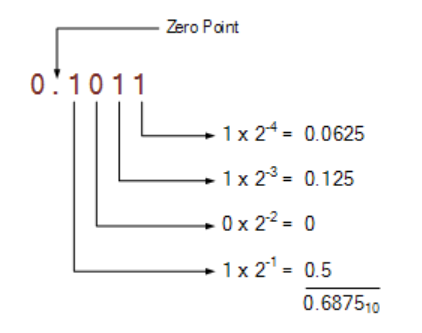
\includegraphics[width=0.8\linewidth]{figures/binary_fraction}
      \caption{Binärerbrüche}
      \label{fig:binaryfraction}
    \end{subfigure}
    \begin{subfigure}{0.4\textwidth}
      \centering
      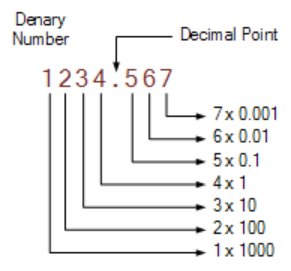
\includegraphics[width=0.6\linewidth]{figures/decimal_fraction}
      \caption{Dezimalbrüche}
      \label{fig:decimalfraction}
    \end{subfigure}
  \end{figure}
  \begin{itemize}
    \item Darstellung \alert{negativer Festkommazahlen}, wobei $d=d_{n}d_{n-1}\ldots d_0\ldots d_{-k}$ mit $\forall i<n:d_i\in Z$ und $d_n\in\{0, 1\}$:
    \begin{itemize}
      \item \alert{möglicherweise negativer Wert} $[d]_{BV} = (-1)^{d_n}\sum_{i=0}^{n-1}\delta(d_i)2^i$ in \alert{Darstellung durch Betrag und Vorzeichen}
      \begin{itemize}
        \item Beispiel 3-Bit Festkommazahlen mit Vorzeichenbit, $n=1$ und $k=1$:
          \begin{table}
            \raggedright
            \begin{tblr}{
                cells = {c, BoxColor},
                column{1} = {PrimaryColor,fg=white},
              }
              $d$                & 10.0 & 10.1 & 11.0 & 11.1 & 00.0 & 00.1 & 01.0 & 01.1 \\
              $[d]_{BV}$ & 0.0  & -0.5 & -1.0 & -1.5 & 0.0   & 0.5 & 1.0  & 1.5 \\
            \end{tblr}
          \end{table}
      \end{itemize}
    \item \alert{möglicherweise negativer Wert} $[d]_{1} = \sum_{i=0}^{n-1}\delta(d_i) 2^i - \delta(d_n)(2^n-2^{-k})$ in \alert{Einerkomplement-Darstellung}
      \begin{itemize}
        \item Beispiel 3-Bit Festkommazahlen mit Vorzeichenbit, $n=1$ und $k=1$:
          \begin{table}
            \raggedright
            \begin{tblr}{
                cells = {c, BoxColor},
                column{1} = {PrimaryColor,fg=white},
              }
              $d$                & 10.0 & 10.1 & 11.0 & 11.1 & 00.0 & 00.1 & 01.0 & 01.1 \\
              $[d]_1$ & -1.5  & -1.0 & -0.5  & 0.0 & 0.0  & 0.5 & 1.0  & 1.5 \\
            \end{tblr}
          \end{table}
      \end{itemize}
      \begin{itemize}
        \item im Negativen hat eine Folge mit mehr $1$en anders als im Positiven betragsmäßig eine kleineren Wert, denn umso mehr $1$en da sind, umso größer wird die Summe $\sum_{i=0}^{n-1}\delta(d_i)2^i$ und umso mehr kann von der subtrahierten größten positiven Zahl $2^n-1$ ausgeglichen werden
        \item um den Wert einer negativen Dezimalzahl binär darzustellen gibt es 2 Methoden
          \begin{description}[abc]
            \item[1.] mit größtmöglichen positven Zahl anfangen $-(2^n-1)$ und überlegen, welche $2$er Potenzen (Stellenwerte) man draufaddieren muss, um die gewünschte Zahl zu erhalten und an den entsprechenden Bits, die diesen $2$er Potenzen entsprechen $1$en setzen
            \item[2.] die passende Ziffernfolge wie gewohnt erstellen, aber mit vertauschten $1$en und $0$en und das Vorzeichenbit ist eine $1$
          \end{description}
      \end{itemize}
      \item \alert{möglicherweise negativer Wert} $[d]_{2} = \sum_{i=0}^{n-1}\delta(d_i)2^i - \delta(d_n)2^n$ in \alert{Zweierkomplement-Darstellung}
      \begin{itemize}
        \item Beispiel 3-Bit Festkommazahlen mit Vorzeichenbit, $n=1$ und $k=1$:
          \begin{table}
            \raggedright
            \begin{tblr}{
                cells = {c, BoxColor},
                column{1} = {PrimaryColor,fg=white},
              }
              $d$                & 10.0 & 10.1 & 11.0 & 11.1 & 00.0 & 00.1 & 01.0 & 01.1 \\
              $[d]_2$ & -2  & -1.5 & -1.0  & -0.5 & 0.0  & 0.5 & 1.0  & 1.5 \\
            \end{tblr}
          \end{table}
      \end{itemize}
      \begin{itemize}
        \item genauso wie beim Einerkomplment bedeuten mehr $1$en im Negativen einen betragsmäßig kleineren Wert
        \item um den Wert einer negativen Dezimalzahl binär darzustellen gibt es 2 Methoden
          \begin{description}[abc]
            \item[1.] mit der größtmöglichen positven Zahl + kleinmöglichen positven Zahl ungleich $0$ anfangen $-(2^n)$ und überlegen, welche $2$er Potenzen (Stellenwerte) man draufaddieren muss, um die gewünschte Zahl zu erhalten und an den entsprechenden Bits, die diesen $2$er Potenzen entsprechen $1$en setzen
            \item[2.] die passende Ziffernfolge wie gewohnt erstellen, aber die kleinstmögliche positve Zahl ungleich $0$ wird als Startwert genommen und die $1$en und $0$en sind vertauscht, sowie das Vorzeichenbit ist eine $1$
          \end{description}
        \item wenn man die kleinste negative Zahl komplementiert: $[10.0]_2' = [01.1]_1 + 1 = [10.0]_2$, dann erhält man erneut die kleinste negative Zahl. Das passt auch ganz gut, da die kleinste negative Zahl im Zweierkomplement keine komplementäre Zahl hat
      \end{itemize}
    \end{itemize}
  \end{itemize}
\end{frame}

% \begin{frame}{Appendix}{Transistoren}
%   \begin{itemize}
%     \item Ströme steuern. Man kann den Stromfluss innerhalb einer elektrischen Schaltung abbremsen, sodass überhaupt kein Strom fließt (der Transistor funktioniert als Schalter). Man kann aber den Stromfluss auch stark beschleunigen, wodurch ein viel stärkerer Strom fließt (der Transistor funktioniert als Verstärker).
%     \item im Kern ist ein Transistor entweder ein strom- oder spannungsgesteuerter Widerstand. Feldeffekttransistoren sind spannungsgesteuerte, Bipolartransistoren sind stromgesteuerte Widerstände.
%     \item Unterschiede bei Art der \alert{Lagungsträger}, die zum Stromfluss beiträgt. Bei einem \alert{Bipolartransistor} sind das Elektronen und Löcher. Daher kommt auch der Teil \enquote{Bi} im Namen. Bei einem \alert{Feldeffekttransistor} sind das hingegen entweder Elektronen oder Löcher, also nur eine Art an Ladungsträger.
%     \item Feldeffekttransistoren werden überwiegend überall dort verwendet, wo hohe Ströme , Bipolartransistoren hingegen dort, wo geringe Ströme fließen.
%   \end{itemize}
% \end{frame}
%
% \begin{frame}[allowframebreaks]{Appendix}{Bipolartransistoren}
% 	\begin{figure}
%     \begin{subfigure}{0.4\textwidth}
%       \centering
%       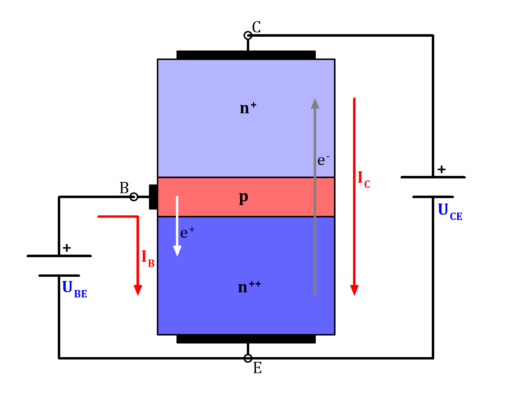
\includegraphics[height=0.5\textheight]{figures/pnp-Transistor}
%       \caption{PNP-Transistor}
%       \label{fig:pnp-transistor}
%     \end{subfigure}
%     \begin{subfigure}{0.4\textwidth}
%       \centering
%       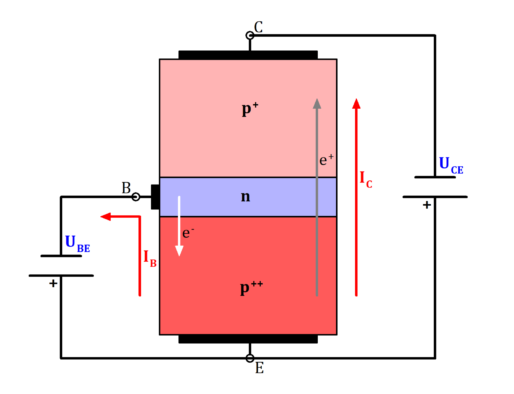
\includegraphics[height=0.5\textheight]{figures/npn-Transistor}
%       \caption{npn-Transistor}
%       \label{fig:npn-transistor}
%     \end{subfigure}
% 	\end{figure}	
%   \begin{itemize}
%     \item \alert{drei Anschlüsse:} Collector (C), Base (B) und Emitter (E) 
%   \end{itemize}
% \end{frame}
%
% \begin{frame}[allowframebreaks]{Appendix}{Feldeffekttransistoren}
%   \begin{figure}
%     % \begin{subfigure}{0.4\textwidth}
%       \centering
%       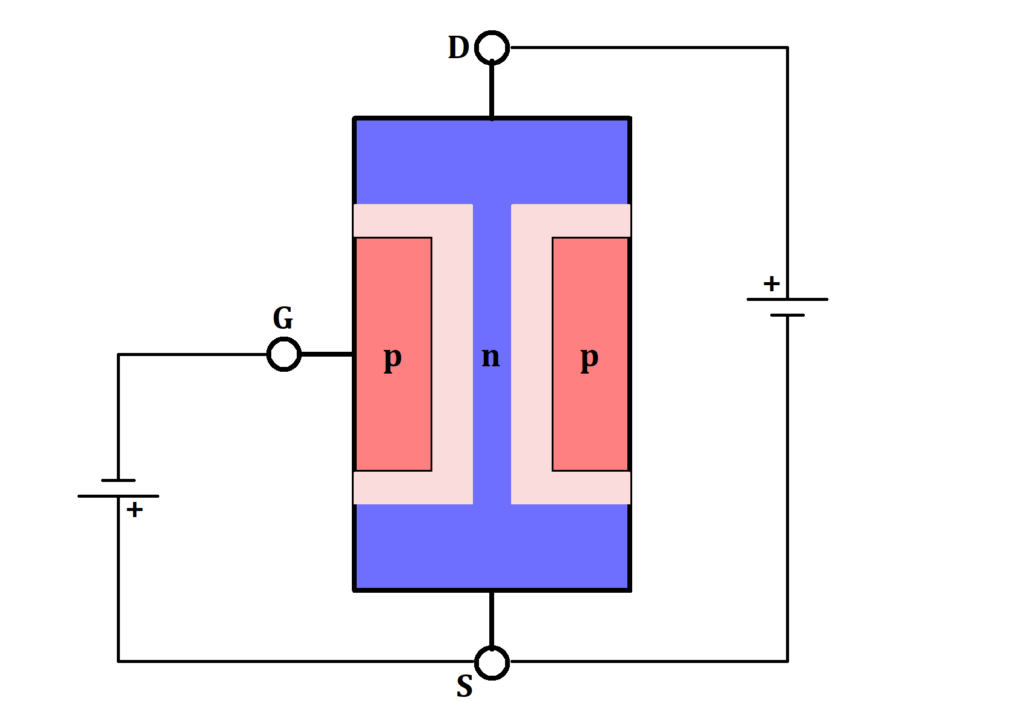
\includegraphics[height=0.5\textheight]{figures/n-Kanal-Feldeffekttransistor.png}
%       \caption{n-Kanal-Feldeffekttransistor}
%     % \end{subfigure}
%     % \begin{subfigure}{0.4\textwidth}
%     %   \centering
%     %   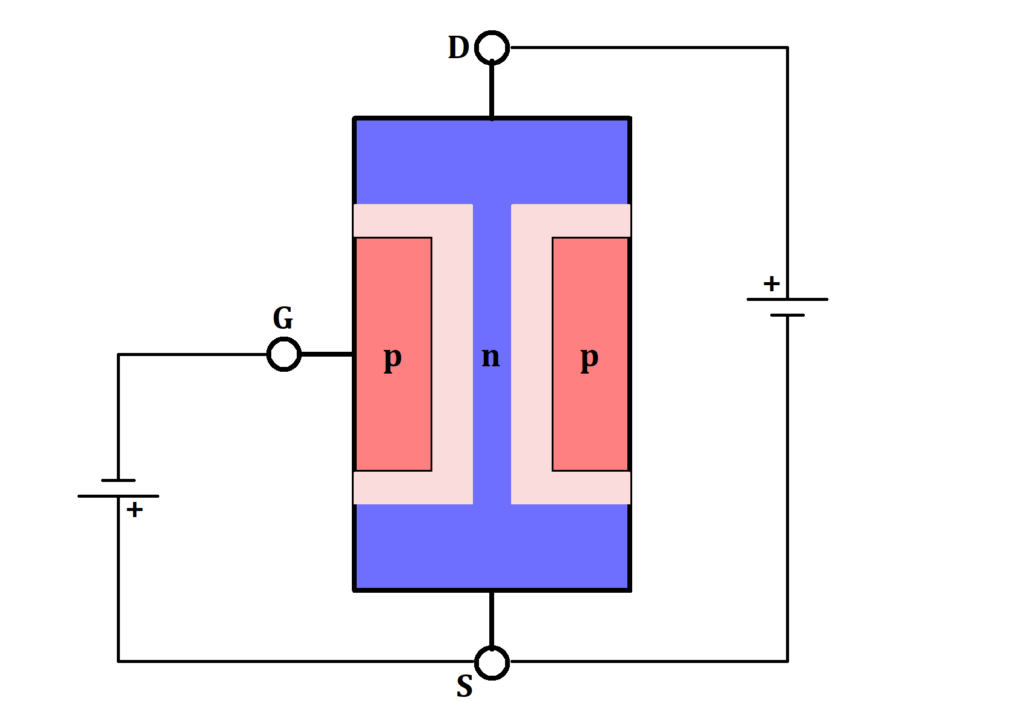
\includegraphics[height=0.5\textheight]{figures/n-Kanal-Feldeffekttransistor.png}
%     %   \caption{p-Kanal-Feldeffekttransistor}
%     % \end{subfigure}
%   \end{figure}
%   \begin{itemize}
%     \item \alert{drei Anschlüsse:} Drain (D, \enquote{Senke, Abfluss}), Gate (G, \enquote{Tor}) und Source (S, \enquote{Quelle, Zufluss})
%     \item Sperrschicht-Feldeffekttransistor (SFET, engl. JFET)
%     \item Je nachdem wie der Kanal, durch denen die Ladungsträger fließen, dotiert ist, findest man die Bezeichnungen n-Kanal-FFET und p-Kanal-FFET
%   \end{itemize}
% \end{frame}
%
% sowohl um wegen keine zweiten 0 die 0 zu überspringen und direkt zu größten negativen Zahl zu springen, aber kann man es sehen, weil jetzt der kleinste Wert $-2^n$ ist und der größte Wert $2^n-1$
